%% Lee
%% In dissertation, change section* to chapter and subsection* to section


\chapter{System Description}
\label{chap-two}

% ----------------------------------------------------------------------------------------------------
% ----------------------------------------------------------------------------------------------------
%\section{ANN System}
%\label{sec:ANN System}

The primary design considerations that drove the architecture of this work are :
\begin{outline}
  \1 Target applications are unable to take advantage of memory reuse opportunities and therefore not able to achieve high performance using local \ac{sram} to store \ac{ann} parameters or the \ac{ann} input 
  \1 \ac{dram} is required for storage of \ac{ann} parameters 
  \1 Target application will likely apply many disparate \acp{ann} to perform various system functions
  \1 Target application will have space and power limitations
\end{outline}

\section{Overview}
\label{sec:chap1_overview}
This work employs \ac{3dic} technology along with a custom 3D-DRAM. The objective was to demonstrate that a pure \ac{3dic} system can implement multiple disparate \acp{ann}. By staying within the \ac{3dic} footprint and taking advantage of high
density \acp{tsv} this work is able to maintain a significantly higher bandwidth over 2D or 2.5D \ac{asic} or \ac{asip} solutions.

The \ac{3dic} system die stack (figure \ref{fig:3DICStack}) includes the 3D-\ac{dram} with a system manager below and one or more processing layers below the manager.
\begin{figure}[!t]
% the [] contains position info e.g. [!t] means here
\centering
\captionsetup{justification=centering}
\captionsetup{width=.9\linewidth}
\centerline{
\mbox{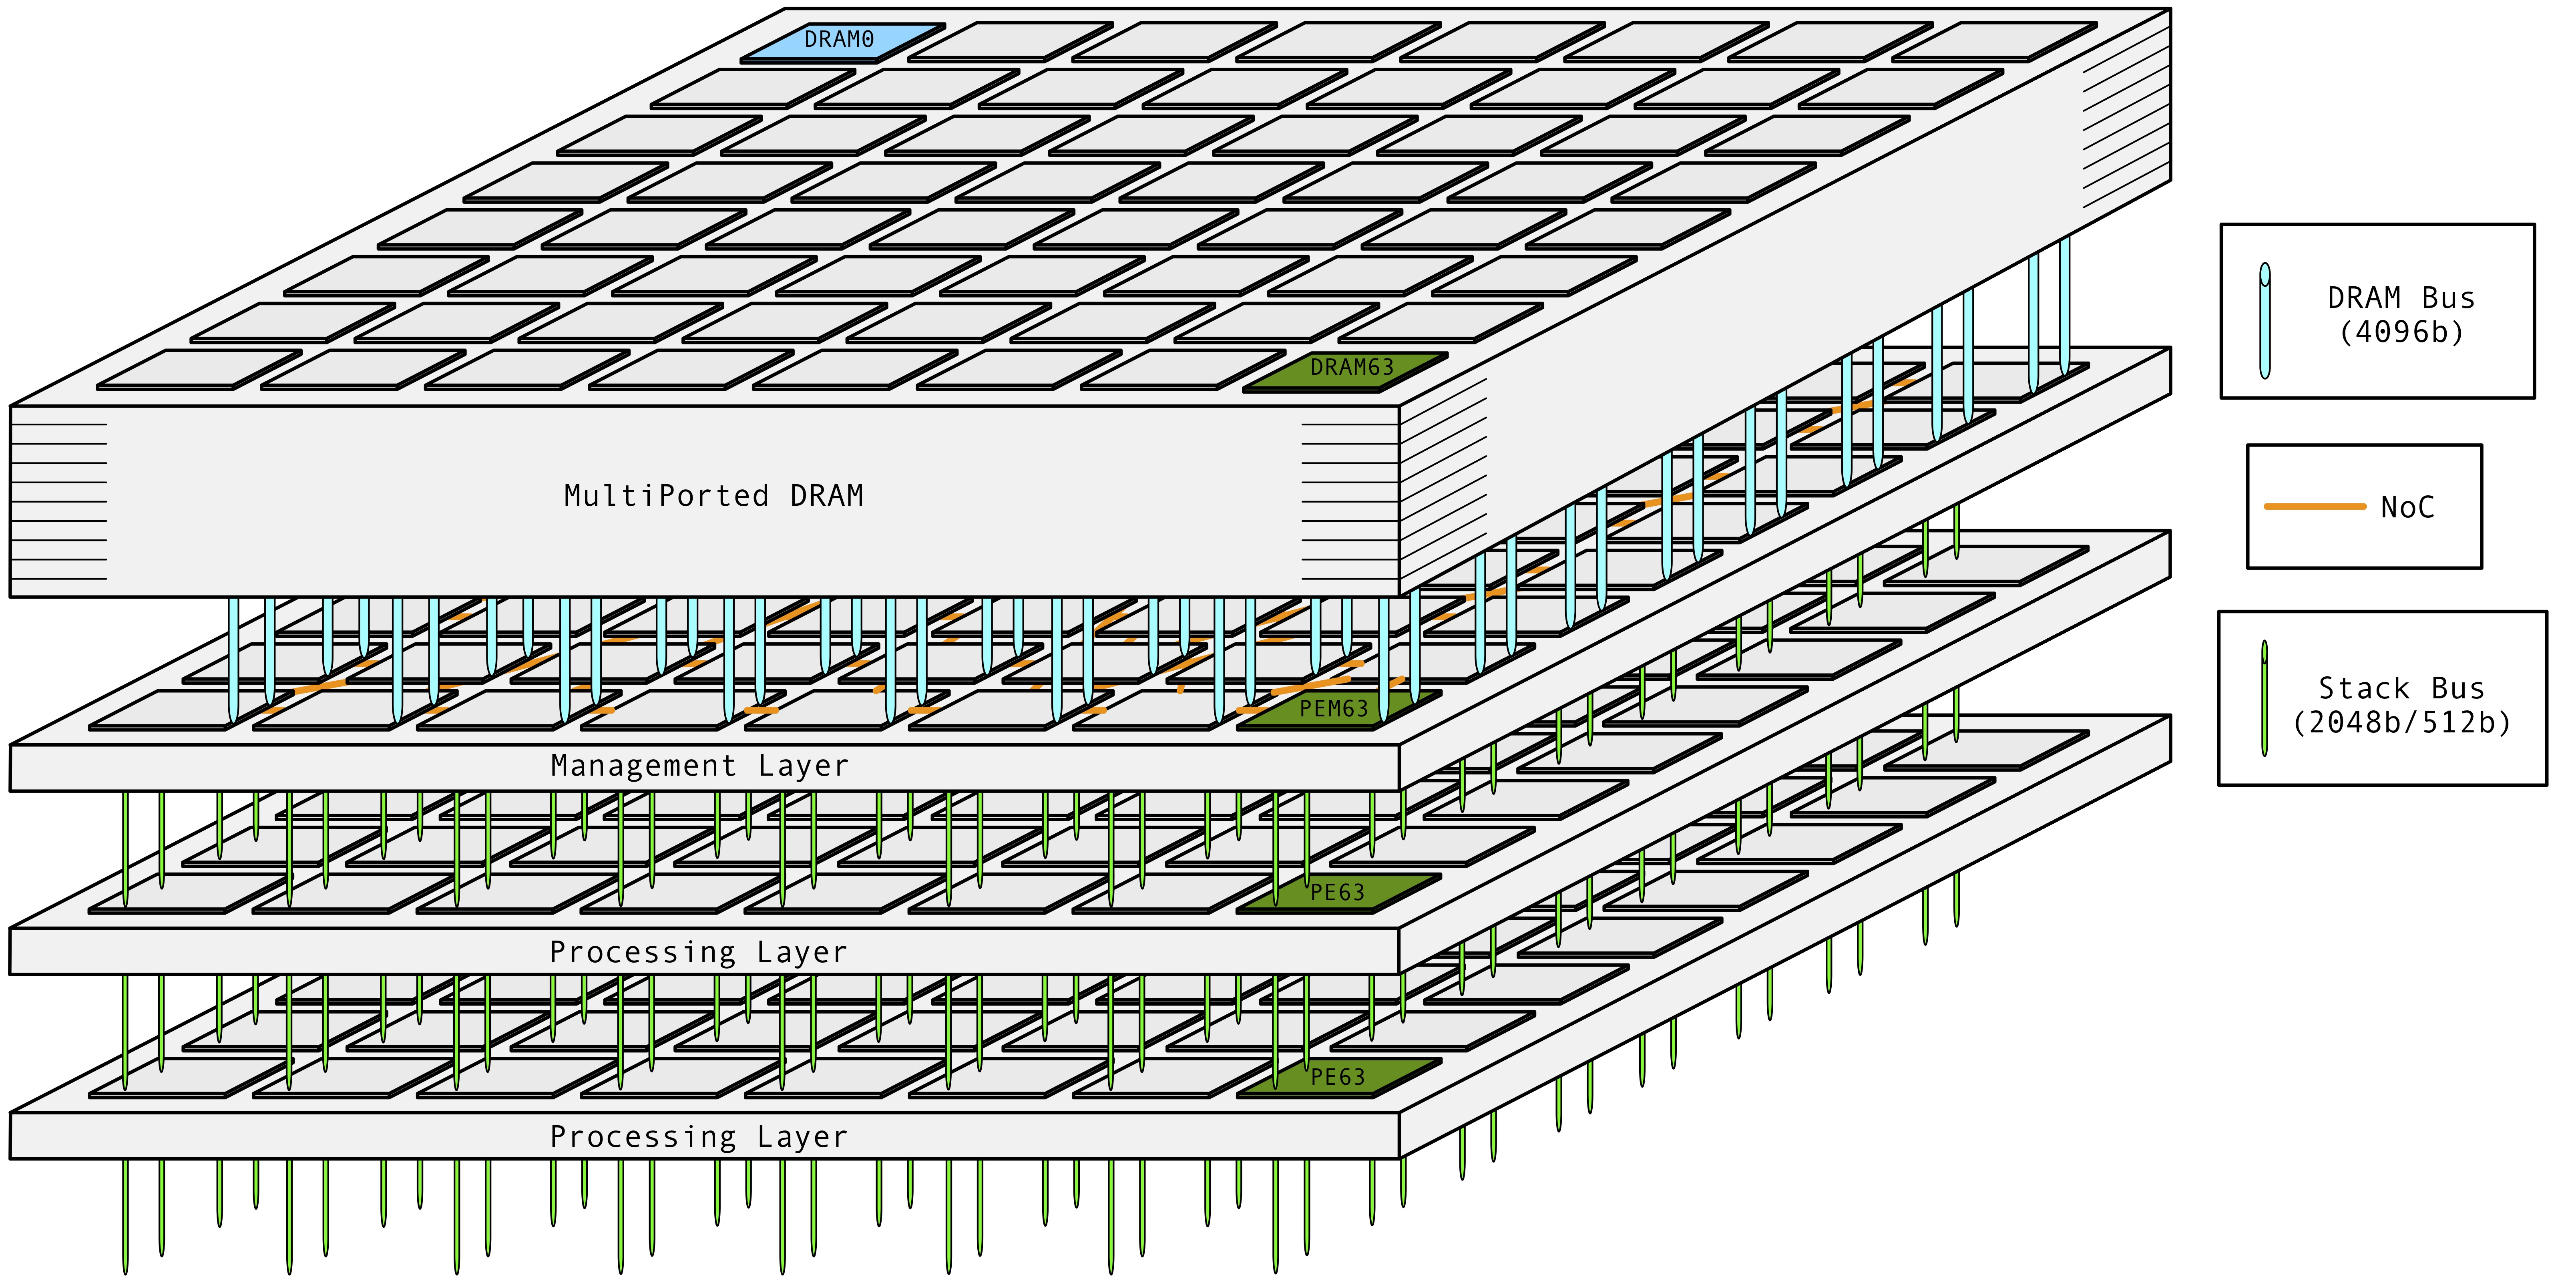
\includegraphics[width=.9\linewidth]{StackDiagram.jpg}}
}
\caption{3DIC System Stack}
\label{fig:3DICStack}
\end{figure}

3D-DRAM has recently become available in standards such as \ac{hbm} and \ac{hmc} and proprietary devices such as the DiRAM4 available from Tezzaron. 
These technologies provide high capacity within a small footprint.

In the case of \ac{hbm} and DiRAM4, the technology can be combined with additional custom layers to provide a system solution.

The question becomes, can a useful system coexist within the same 3D footprint?

This work targeted a baselne system with:
\begin{itemize}
  \item Computations require single precision floating point precision
  \item Utilize the Tezzaron DiRAM4 \ac{dram} for for main memory
\end{itemize}
The work includes customizing the interface to a 3D-\ac{dram}, researching data structures to describe storage of \ac{ann} parameters, designing a memory manager with unique micro-coded instructions and a \ac{pe} layer.  
The system is designed such that a sub-system, known as a \ac{ssc} operates on one of these disjoint memories within the 3D-\ac{dram} (see figure \ref{fig:diram4Layout}).

When the \acp{ssc} need to share data or neuron activations, the data is passed between \acp{ssc} using a \ac{noc}.

An overview of the various blocks and interconnects are given below:

% ----------------------------------------------------------------------------------------------------
\section{3D-DRAM}
The targetted 3D-\ac{dram}, the Tezzaron DiRAM4 is a 3D-\ac{dram} employs multiple memory array layers in conjunction with a control and IO layer.
The memory is formed from 64 disjoint sub-memories each providing upwards of 1Gigabit with a total capacity of at least 64 gigabit.
\begin{figure}[!t]
% the [] contains position info e.g. [!t] means here
\centering
\captionsetup{justification=centering}
\captionsetup{width=.9\linewidth}
\centerline{
\mbox{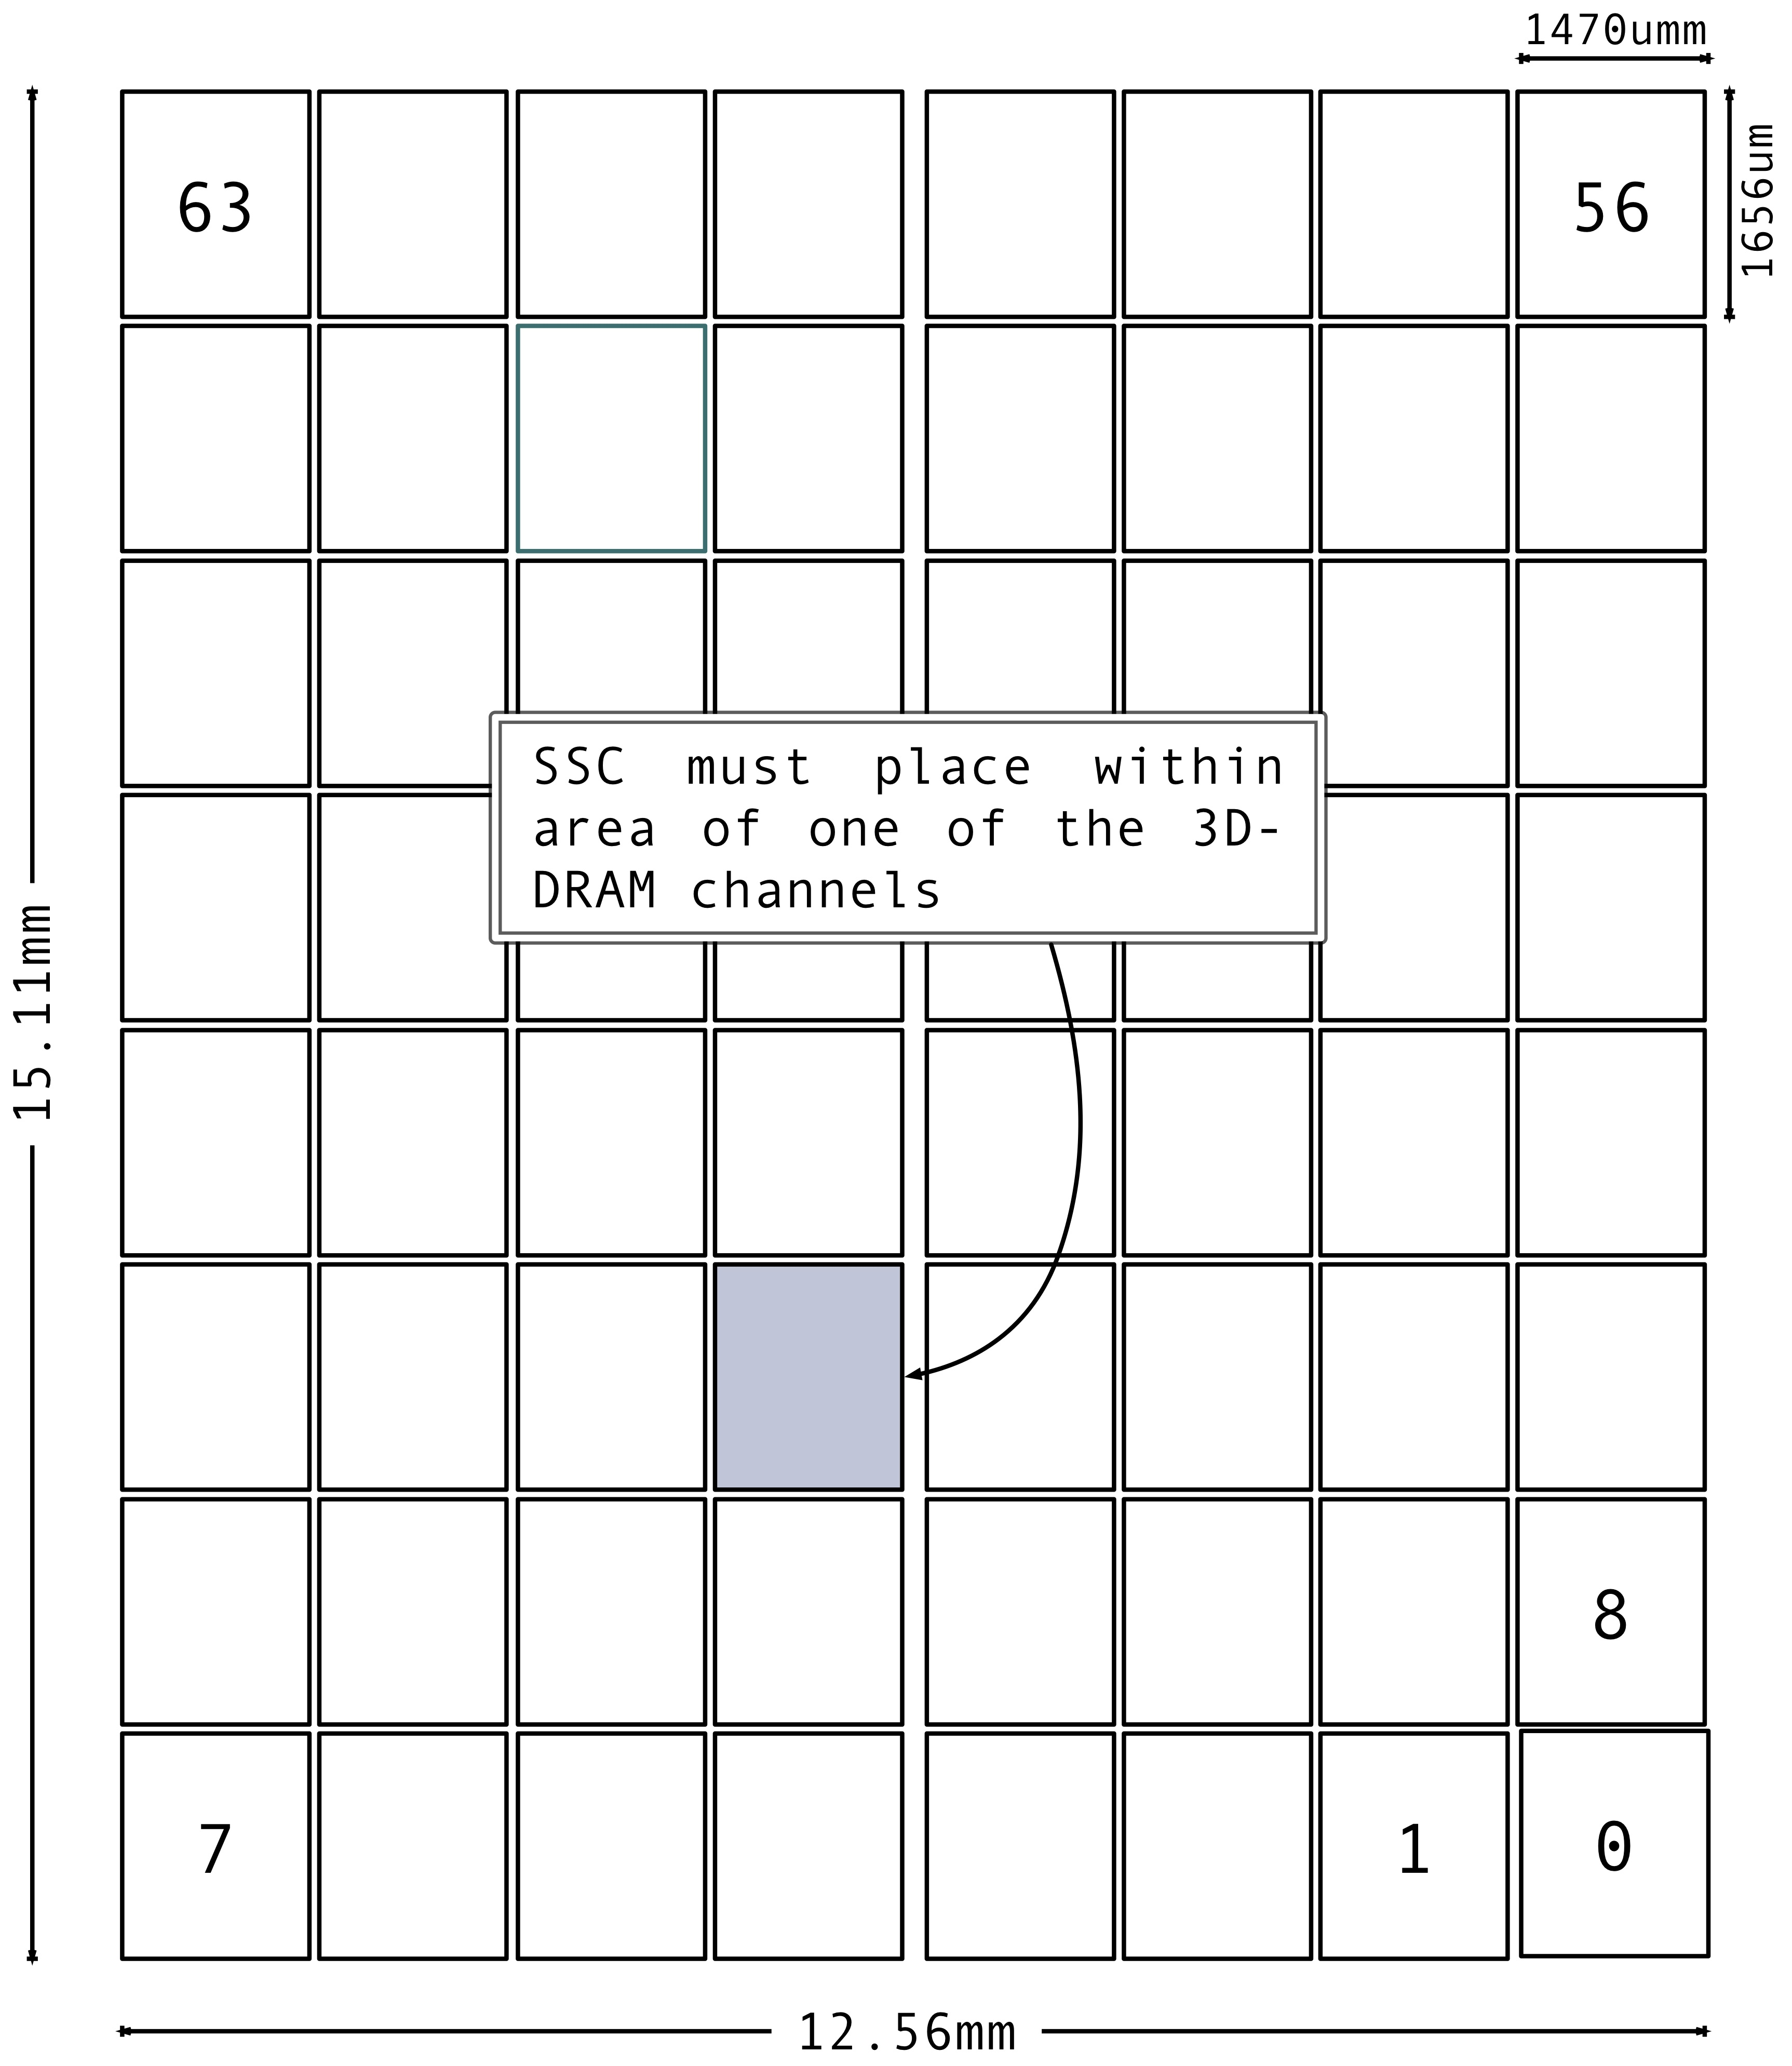
\includegraphics[width=.6\linewidth]{DiRAM4Layout.jpg}}
}
\caption{\ac{dram} Physical Interface Layout showing area for \ac{ssc}}
\label{fig:diram4Layout}
\end{figure}


% ----------------------------------------------------------------------------------------------------
\section{Manager Layer}
The Manager block is the main controller in the system. The operations required to process an \ac{ann} are formed from individual instructions which are decoded by the Manager. 
These instructions include descriptors to describe memory read operations, processing engine operations and memory write operations. The manager reads these system instructions from an instruction memory, decodes the instruction and configures the various blocks in the system.
The configuration includes:
\begin{itemize}
      \item initiate operand reads from \ac{dram}
      \item prepare the processing engine (\ac{pe}) to operate on the operands
      \item prepare the result processing engine to take the resulting neuron activations from the \ac{pe} and write those results back to the \ac{dram}
      \item replicate the resulting neuron activation's to neighbor managers for processing of other \ac{ann} layers
\end{itemize}

% ----------------------------------------------------------------------------------------------------
\section{Processing Layer}
\label{ssec:Processing Layer}
The \ac{pe} is able to operate on data streamed directly from the \ac{dram} via the Manager layer. The \ac{pe} is configured by the manager to perform operations on the operand data streamed from the manager. In the baseline system, the main operation is to perform multiply-accumulates on 32 execution lanes of two operands. These operands typically are the pre-synaptic neuron activation's and the connection weights. The \ac{pe} also performs the activation function on the result of the MAC to generate the neuron activation value. These 32 activation values are sent back to the Manager layer.

% ----------------------------------------------------------------------------------------------------
\section{Layer Interconnect}
\label{ssec:Layer Interconnect}

The layers are connected using through-silicon-vias (\ac{tsv}s) which provide high connection density, high bandwidth and low energy.
By ensuring the system stays within the 3D footprint ensures we can take advantage of the huge benefits provided by \ac{tsv}s.

% ----------------------------------------------------------------------------------------------------
\section{Inter-Manager Communication}
\label{ssec:Inter-Manager Communication}

During configuration and/or computations, data must be transported between managers. This inter-manager communication is provided by an \ac{noc}.
When computing an \ac{ann} across multiple processing sub-systems, often neuron activation data must be shared between these \ac{ssc}s. The \ac{ssc} includes the \ac{dram} port, the manager and the \ac{pe}. An \ac{noc} within each management block communicates with each adjacent manager using a mesh network. This \ac{noc} has a forwarding table that can be reconfigured to provide more efficient routing for a given processing step.

A control and data flow diagram of the stack showing the 64 sub-system columns can be seen in figure \ref{fig:FlowDiagram}.
\begin{figure}[!t]
% the [] contains position info e.g. [!t] means here
\centering
\captionsetup{justification=centering}
\centerline{
\mbox{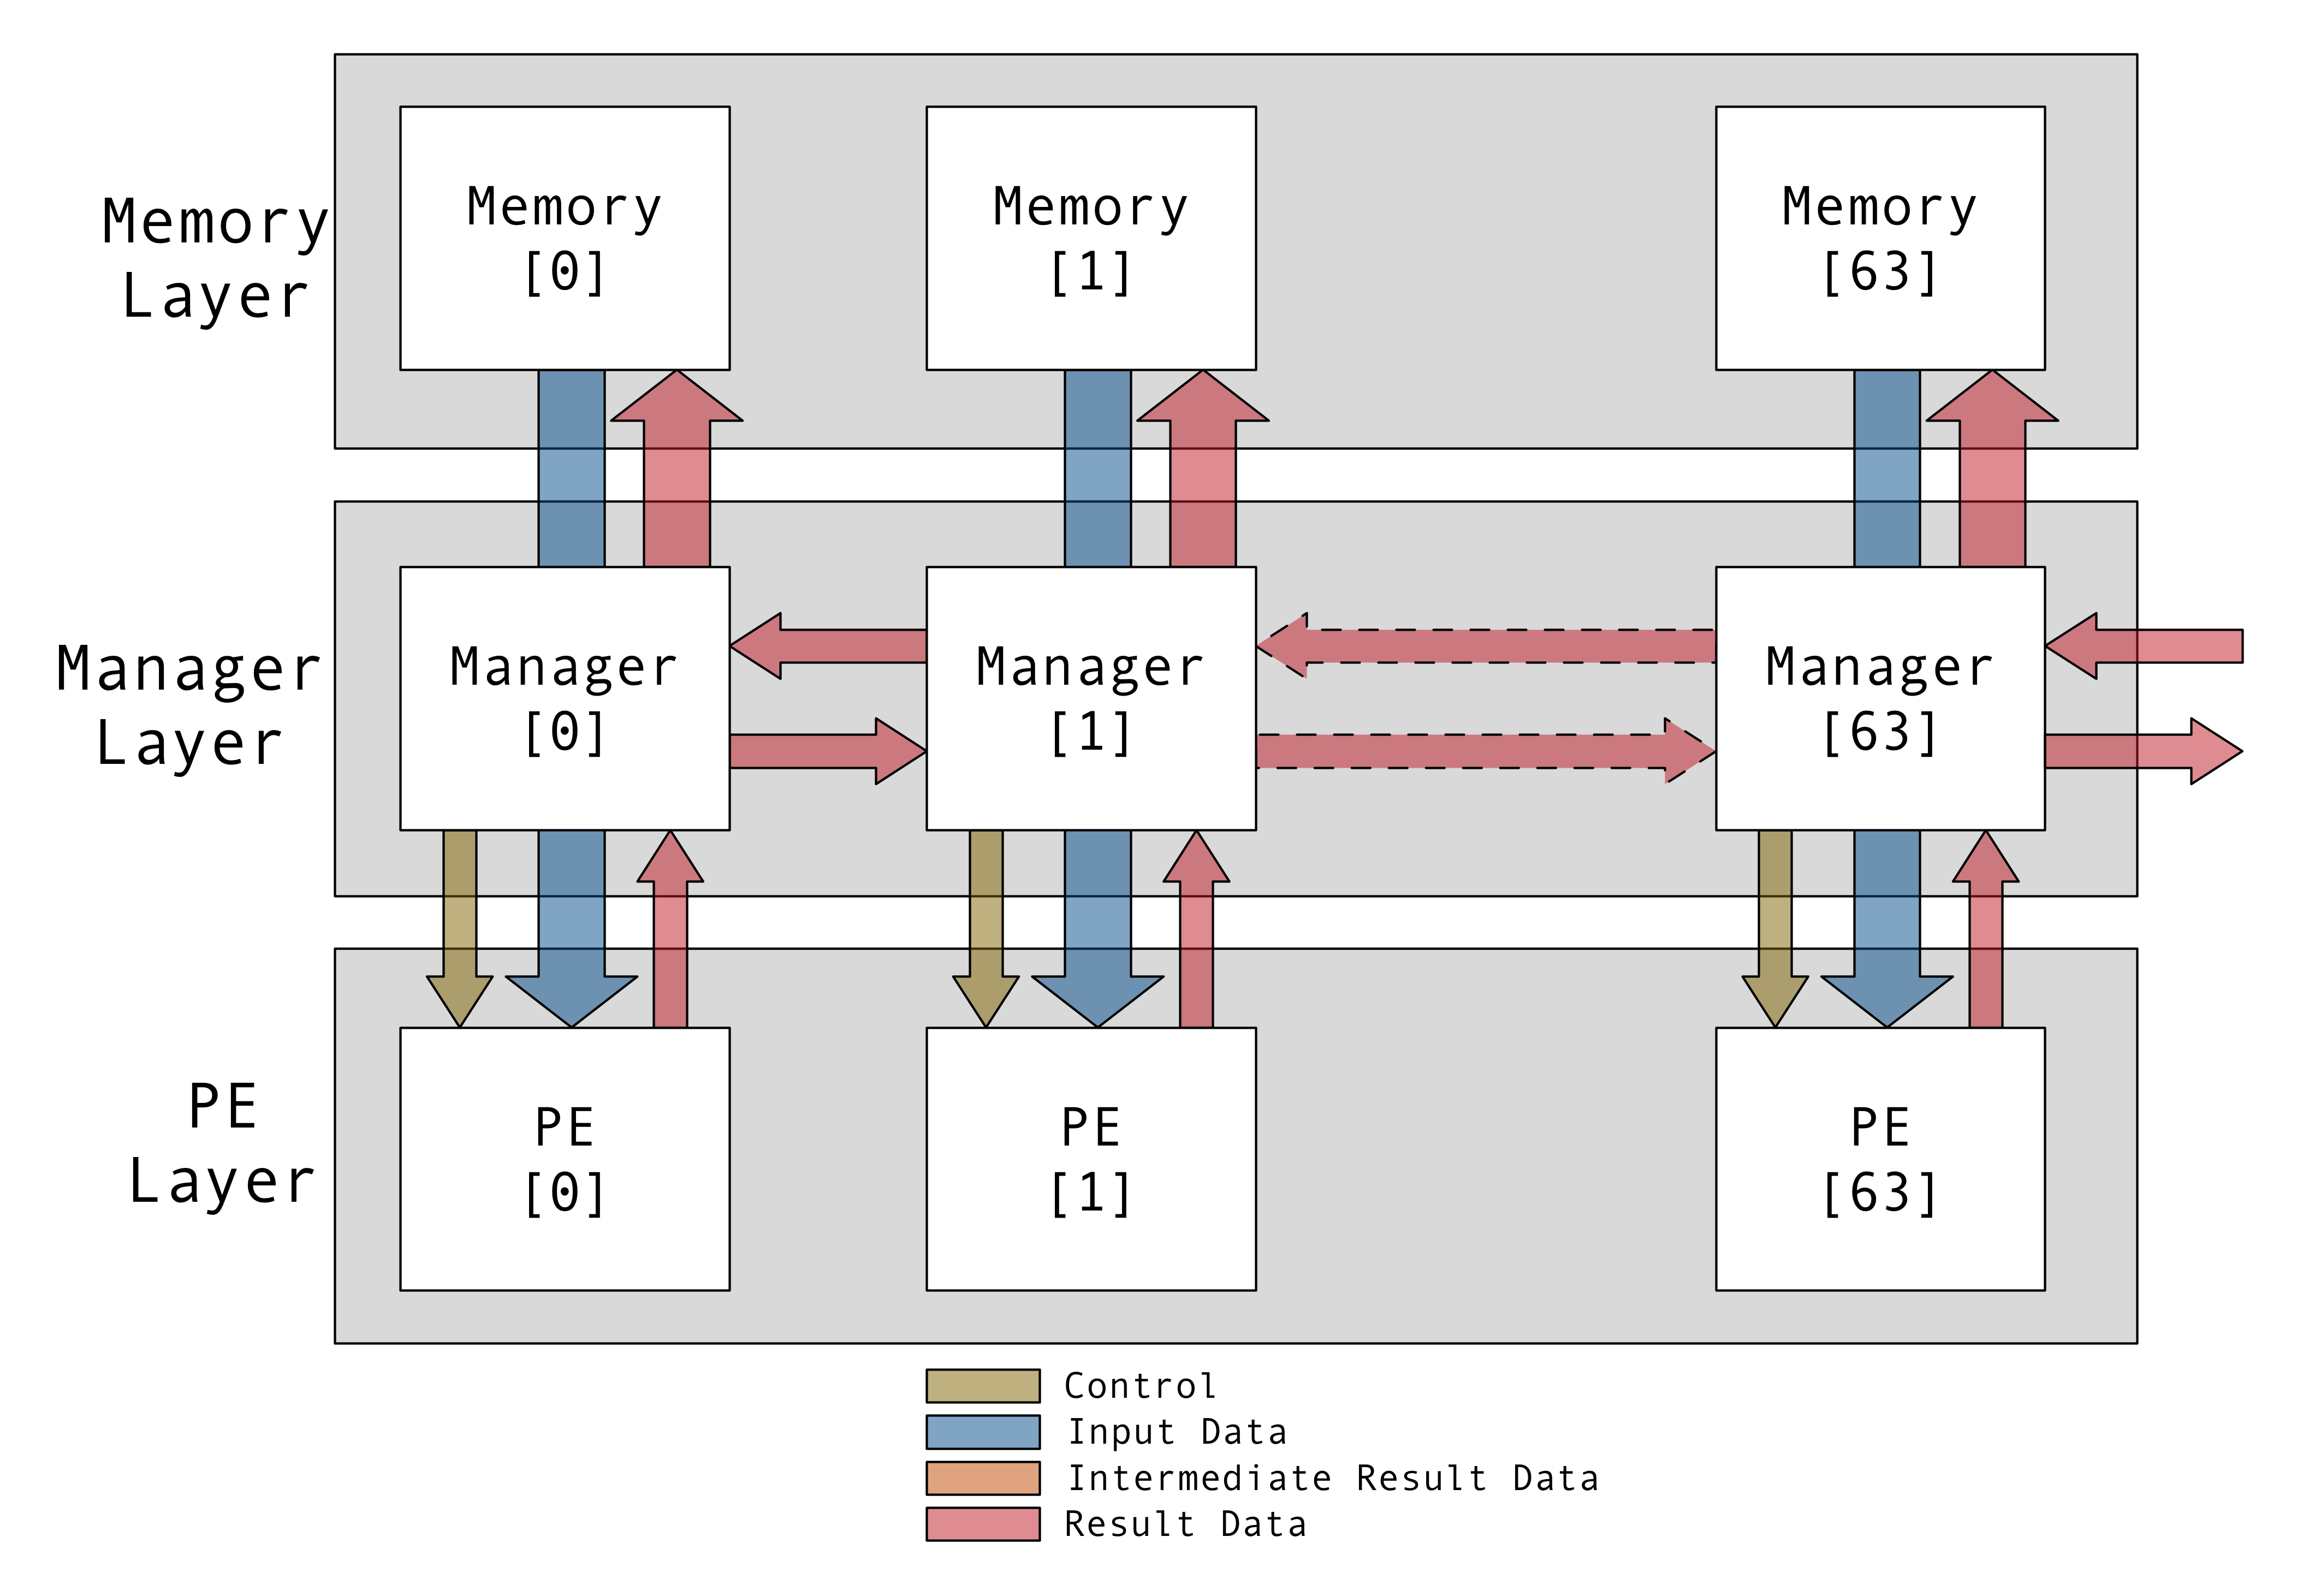
\includegraphics[width=.8\linewidth]{FlowDiagram.jpg}}
}
\caption{System Flow Diagram}
\label{fig:FlowDiagram}
\end{figure}


